
\subsection*{Review of Parametric Notation}

{\ttfamily
\fontdimen2\font=0.4em
\fontdimen3\font=0.2em
\fontdimen4\font=0.1em
\fontdimen7\font=0.1em
\hyphenchar\font=`\-

\hypertarget{scripts_vectors_in_space_n_vectors_parametric}{The equation}  for a plane in three variables $x$, $y$ and $z$ looks like
\[
ax+by+cz=d
\]
where $a$, $b$, $c$, and $d$ are constants.
Lets look at the example
\[
x+2y+5z=3\, .
\]
In fact this is a system of linear equations whose solutions form  a plane with normal vector $(1,2,5)$.
As an augmented matrix the system is simply
\[
\Big( 1 \ \ 2 \ \ 5\ \Big| \ 3 \Big)\, .
\]
This is actually RREF! So we can let $x$ be our pivot variable and $y$, $z$ be represented
by free parameters $\lambda_1$ and $\lambda_2$:
\[
x=\lambda_1\, , \qquad y = \lambda_2\, .
\]
Thus we write the solution as
\[
\begin{array}{ccccc}
x&=&-2\lambda_1&-5\lambda_2&+3\\
y&=&\lambda_1&&\\
z&=&&\lambda_2&
\end{array}
\]
or in vector notation
\[
\begin{pmatrix}
x\\y\\z
\end{pmatrix}
=
\begin{pmatrix}
3\\0\\0
\end{pmatrix}
+\lambda_1
\begin{pmatrix}
-2\\1\\0
\end{pmatrix}
+\lambda_2
\begin{pmatrix}
-5\\0\\1
\end{pmatrix}\, .
\]
This describes a plane parametric equation. Planes are ``two-dimensional'' because they are 
described by two free variables. Here's a picture of the resulting plane:
\begin{center}
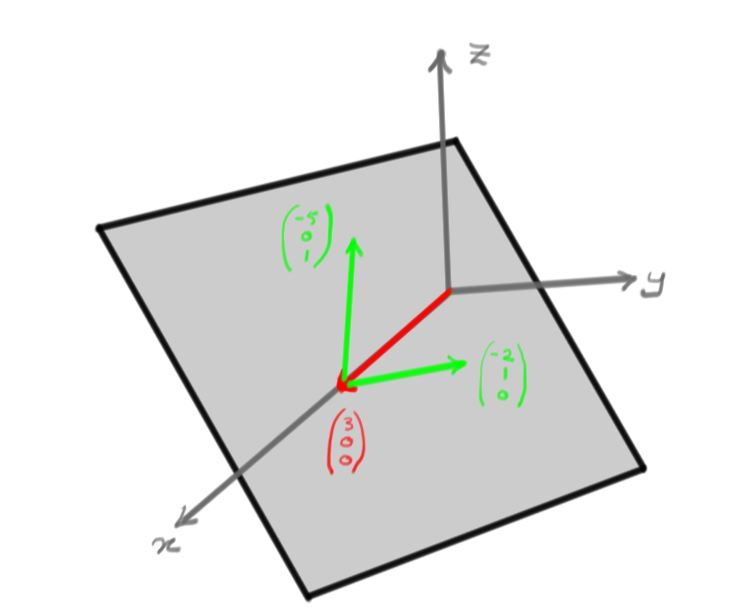
\includegraphics[alt={A plane in space through the point (3,0,0) that contains the vectors (-5,0,1) and (-2,1,0).},scale=.35]{katrinas_plane.jpg}
\end{center}

} % Closing brace for the font

%\newpage
